\chapter{Brief Compendium of Neutron Diffusion Benchmarks}
\label{ap:benchmarks}

\section{Introduction}
\section{Two Dimension}
  \subsection{VVER440}
    \begin{figure}
      \centering
      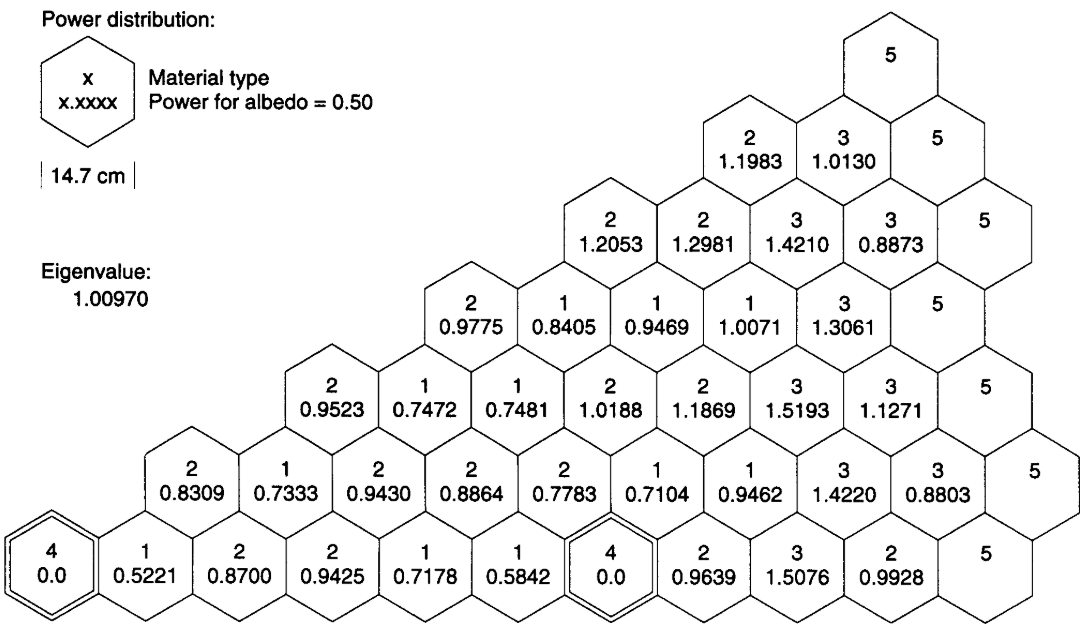
\includegraphics[width=0.6\textwidth]{vver440_geom}
      \caption{VVER440 Geometry \cite{chao}.}
      \label{fig:vver440_geom}
    \end{figure}
    \begin{table}
      \caption{VVER440 Cross Sections.}
      \label{tab:vver440xs}
      \begin{center}
        \begin{tabular}{cccccc}
          \toprule
          &MAT1&MAT2&MAT3&MAT4&MAT5\\
          \midrule
          $D_1$&1.346600E+00&1.337700E+00&1.332200E+00&1.195300E+00&1.448500E+00\\
          $D_2$&3.716900E-01&3.691800E-01&3.650200E-01&1.931300E-01&2.517600E-01\\
          $\Sigma_{r1}$&2.525500E-02&2.470900E-02&2.435000E-02&3.563600E-02&3.318400E-02\\
          $\Sigma_{r2}$&6.427700E-02&7.936100E-02&1.001000E-01&1.349800E-01&3.283900E-02\\
          $\Sigma_{s 1\rightarrow 2}$&1.689300E-02&1.591200E-02&1.488800E-02&2.226400E-02&3.226200E-02\\
          $ \nu \Sigma_{f1}$&4.448800E-03&5.533700E-03&7.039100E-03&&\\
          $ \nu \Sigma_{f2}$&7.375300E-02&1.058100E-01&1.496400E-01&&\\
          \bottomrule
        \end{tabular}
      \end{center}
    \end{table}
  \subsection{SNR}
    \begin{figure}
      \centering
      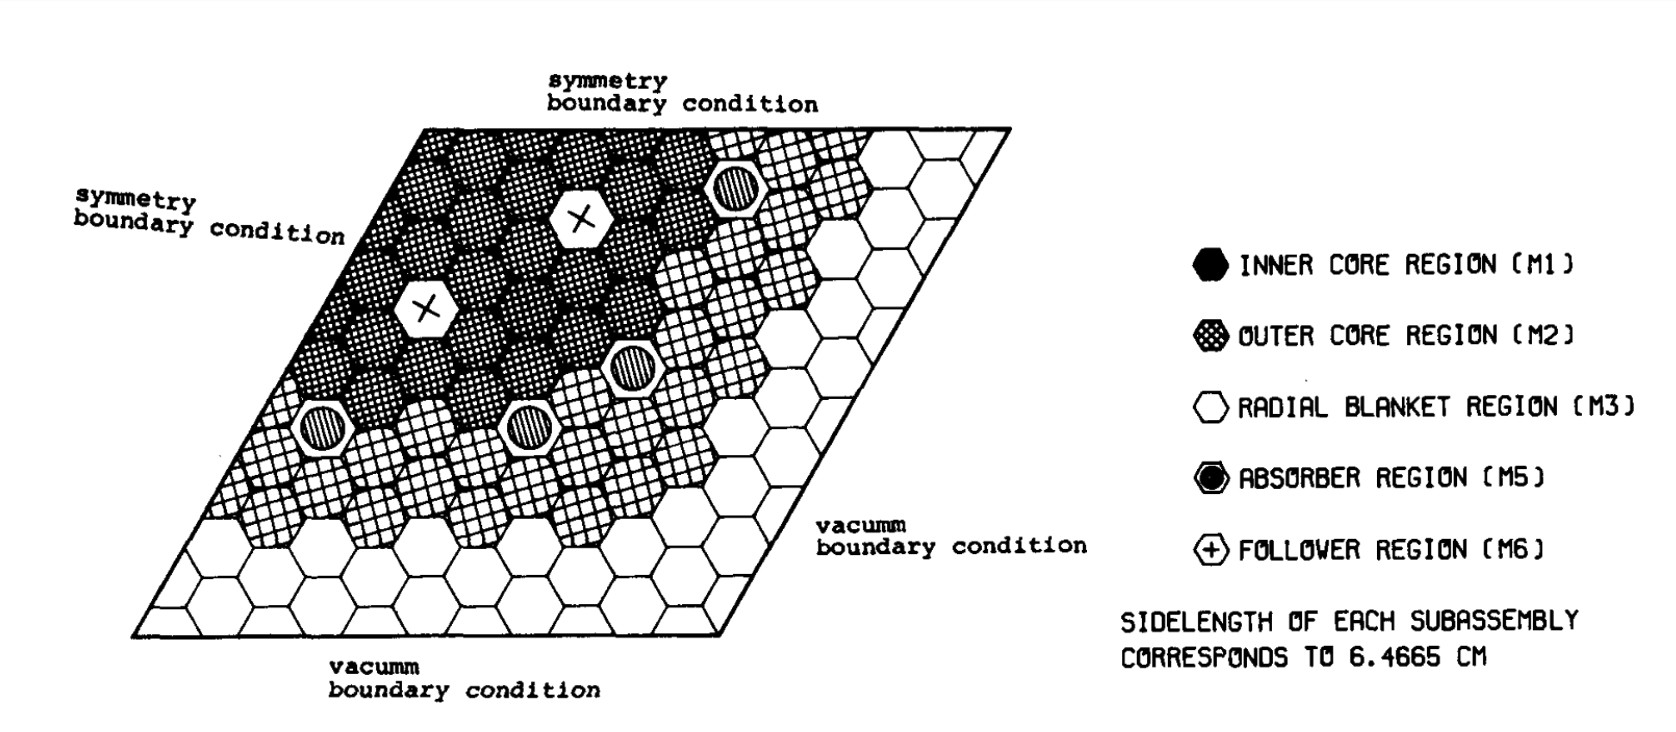
\includegraphics[width=0.6\textwidth]{snr_geom}
      \caption{SNR Geometry \cite{argonneBenchmark}.}
      \label{fig:snr_geom}
    \end{figure}
    \begin{table}
      \caption{SNR Cross Sections.}
      \label{tab:snrxs}
      \begin{center}
        \begin{tabular}{ccccccc}
          \toprule
          &I1&I2&I3&I4&I5&I6\\
          \midrule
          $D_1$&2.876787E+00&2.876539E+00&2.285610E+00&2.716653E+00&2.503066E+00&4.616422E+00\\
          $D_2$&1.570845E+00&1.571363E+00&1.171935E+00&1.440943E+00&1.314665E+00&2.901831E+00\\
          $D_3$&7.224859E-01&7.127076E-01&6.324751E-01&7.203469E-01&5.742770E-01&1.021179E+00\\
          $D_4$&9.641993E-01&9.429781E-01&8.183574E-01&9.876836E-01&6.153695E-01&1.729625E+00\\
          $\Sigma_{r1}$&2.820400E-02&2.878200E-02&3.595900E-02&2.909300E-02&2.481400E-02&1.315900E-02\\
          $\Sigma_{r2}$&5.274700E-03&6.049100E-03&5.885500E-03&4.490900E-03&1.641200E-02&1.455900E-03\\
          $\Sigma_{r3}$&1.761200E-02&1.951000E-02&1.604100E-02&1.308200E-02&7.212200E-02&4.600100E-03\\
          $\Sigma_{r4}$&2.654600E-02&3.371400E-02&1.334900E-02&9.956200E-03&1.686800E-01&7.866000E-04\\
          $\Sigma_{s 1\rightarrow 2}$&2.359700E-02&2.326200E-02&3.207100E-02&2.632200E-02&2.294600E-02&1.294200E-02\\
          $\Sigma_{s 1\rightarrow 3}$&4.079100E-06&4.645100E-06&3.888000E-06&2.890700E-06&1.032000E-06&6.878000E-07\\
          $\Sigma_{s 2\rightarrow 3}$&1.615300E-03&1.571800E-03&2.777600E-03&2.288900E-03&3.768700E-03&1.287100E-03\\
          $\Sigma_{s 1\rightarrow 4}$&4.449300E-08&4.996800E-08&4.503900E-08&3.324800E-08&1.048900E-08&6.990300E-09\\
          $\Sigma_{s 2\rightarrow 4}$&4.230900E-08&4.072400E-08&9.001800E-08&6.213300E-08&7.036100E-12&4.363300E-12\\
          $\Sigma_{s 3\rightarrow 4}$&4.683800E-03&4.341400E-03&5.897100E-03&5.353600E-03&8.681500E-03&3.453300E-03\\
          $ \nu \Sigma_{f1}$&1.187800E-02&1.494300E-02&7.742700E-03&5.427900E-03&&\\
          $ \nu \Sigma_{f2}$&5.325200E-03&7.688700E-03&1.082500E-04&7.585700E-05&&\\
          $ \nu \Sigma_{f3}$&1.047100E-02&1.480900E-02&2.974200E-04&2.121799E-04&&\\
          $ \nu \Sigma_{f4}$&2.661100E-02&3.815900E-02&8.468699E-04&5.759200E-04&&\\
          \bottomrule
        \end{tabular}
      \end{center}
    \end{table}
  \subsection{IAEA}
    \begin{figure}
      \centering
      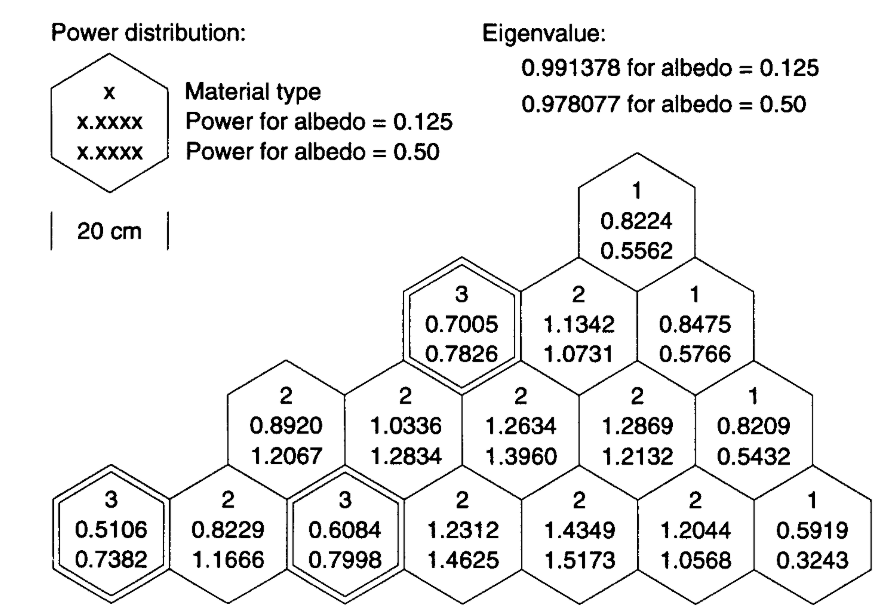
\includegraphics[width=0.6\textwidth]{iaea_nore_geom}
      \caption{IAEA Without Reflector Geometry \cite{chao}.}
      \label{fig:iaea_nore_geom}
    \end{figure}
    \begin{figure}
      \centering
      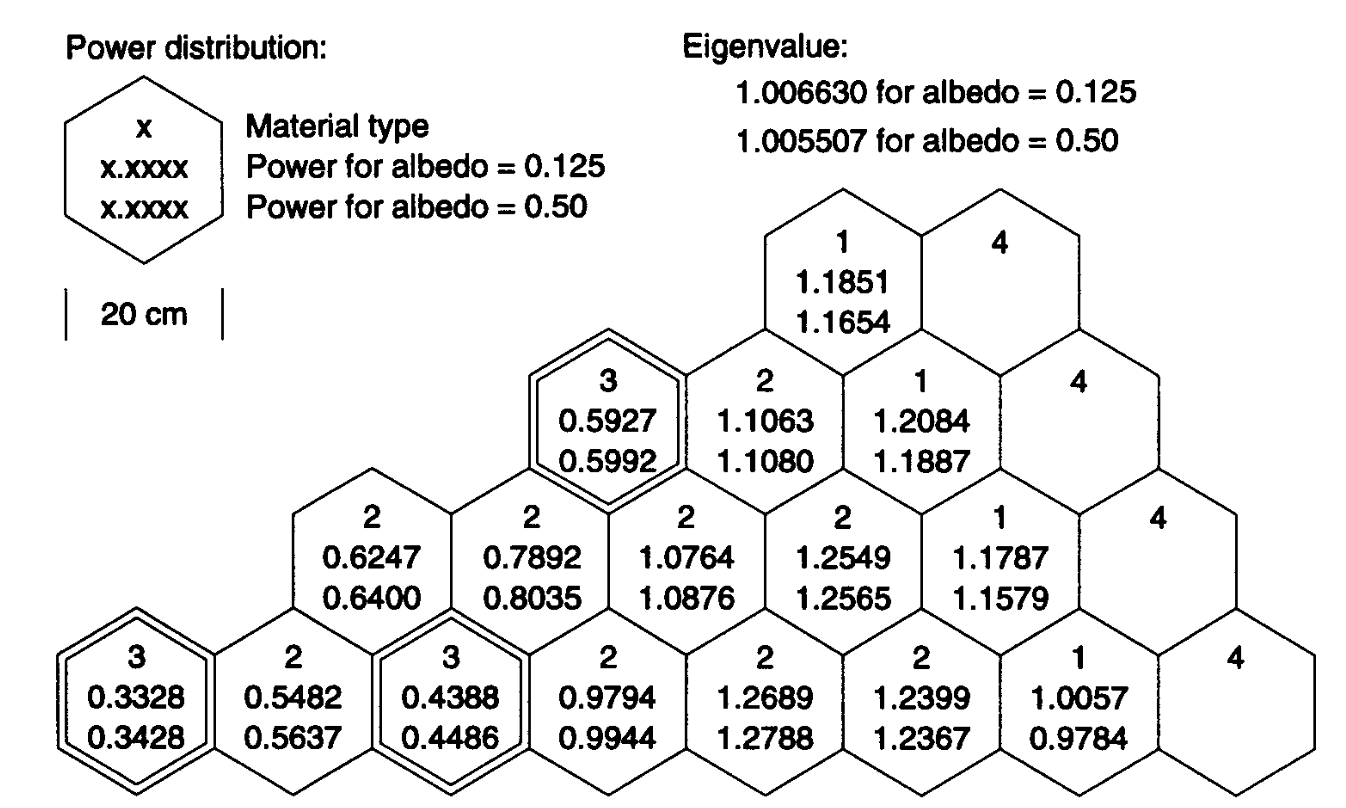
\includegraphics[width=0.6\textwidth]{iaea_refl_geom}
      \caption{IAEA With Reflector Geometry \cite{chao}.}
      \label{fig:iaea_refl_geom}
    \end{figure}
    \begin{table}
      \caption{IAEA Cross Sections.}
      \label{tab:iaeaxs}
      \begin{center}
        \begin{tabular}{ccccc}
          \toprule
          &MAT1&MAT2&MAT3&REFL\\
          \midrule
          $D_1$&1.500001E+00&1.500000E+00&1.500001E+00&1.500000E+00\\
          $D_2$&4.000001E-01&4.000000E-01&4.000001E-01&4.000000E-01\\
          $\Sigma_{r1}$&3.000000E-02&3.000000E-02&3.000000E-02&4.000000E-02\\
          $\Sigma_{r2}$&8.000000E-02&8.500000E-02&1.300000E-01&1.000000E-02\\
          $\Sigma_{s 1\rightarrow 2}$&2.000000E-02&2.000000E-02&2.000000E-02&4.000000E-02\\
          $ \nu \Sigma_{f1}$&&&&\\
          $ \nu \Sigma_{f2}$&1.350000E-01&1.350000E-01&1.350000E-01&\\
          \bottomrule
        \end{tabular}
      \end{center}
    \end{table}
\section{Three Dimension}
  \subsection{MONJU}
  \subsection{KNK}

